% !TEX root = Master.tex

To start things off, a look at the scatterplot in \autoref{fig:scatter_res_kcc_26} between the residuals of \ac{KCC} 2 \& \ac{KCC} 6 provides a first hint of a potential correlation structure. For the most part, the data look quite elliptically scattered. Thus, a normal or a t-copula might be appropriate copulas to be used.
\\


\begin{figure}[H]
\centering
  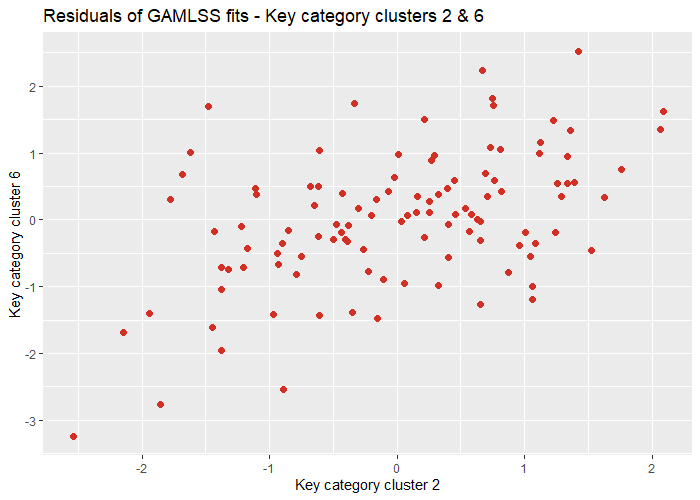
\includegraphics[width=0.45\linewidth]{figures/scatter_res_kcc_26.png}
  \caption{Scatterplot of estimated residuals of GAMLSS fits for key category clusters 2 \& 6}
  \label{fig:scatter_res_kcc_26}
\end{figure}

With the help of the function \textit{BiCopSelect()} of the R package \textit{VineCopula} \citep{nagler2019vinecopula}, we can select an appropriate bivariate copula family for the data. A set of possible copula families is considered and maximum likelihood estimations for each are carried out. Selection of a bivariate copula is based on the lowest \ac{AIC}. The normal and the t-copula are the first in the family set. The selected copula is a t-copula with 3.17\footnote{Estimation returns degrees of freedom as positive real values above 2 instead of just integer values.} \ac{dof} and the Pearson's rho as well as Kendall's tau correlation coefficients coincide with the empirical sample coefficients of 0.49 and 0.3 respectively.
\\

Furthermore, to estimate the copula parameter flexibly over time, the \ac{GJRM} framework introduced by \cite{marra1605bivariate} is utilized\footnote{See Section \ref{ssec:conditional_copulas} as well as the referred paper.}. Essentially, the scope of the \ac{GAMLSS} framework is extended to a bivariate copula additive model, where all parameters of the margins as well as the copula parameter can be estimated simultaneously using structured additive predictors. The parameters are estimated within a penalized likelihood framework using a trust region algorithm with integrated automatic smoothing parameter selection (More details can be found in the referenced literature). This framework has been implemented in R by \cite{marragjrm} within the scope of the \textit{gjrm} package. \\

With the \ac{GAMLSS} fit residuals of the key category clusters 2 \& 6 acting as marginal inputs, normal distributions for both and a t-copula with the above mentioned degrees of freedom as starting value, the formula specification is as follows: \\



\begin{equation}
\begin{array}{c}
\mu_{KCC 2}=\beta_{\mu,KCC2} \qquad \mu_{KCC 6}=\beta_{\mu,KCC6}  \\  \noalign{\vskip5pt}

log(\sigma_{KCC 2})=\beta_{\sigma,KCC2} \qquad log(\sigma_{KCC 6})=\beta_{\sigma,KCC6} \\  \noalign{\vskip5pt}

log(\nu) = \beta_{\nu} \\  \noalign{\vskip5pt}

tanh^{-1}(\theta)=\beta_{\theta} + \textit{promo\_type} +f(\textit{time}),
\end{array}
\label{eq:gjrm_formula_26}
\end{equation} \\

where $\nu$ denotes the degrees of freedom of the t-copula, $tanh^{-1} = $ is the inverse hyperbolic tangent function\footnote{Defined as $\tanh ^{-1} (x)=\frac{1}{2} \ln \left(\frac{1+x}{1-x}\right)$ on the domain $ \{ x \in \mathbb{R}:-1<x<1\}$.} relating the expected value of the copula parameter $\hat{\theta}$ to the additive predictor $\beta_{\theta}+f\left(t_{time}\right)$ and $f$ being a smooth function build upon thin plate regression splines and 30 equidistant knots. Note that as the chosen copula is a Student's t-copula, $\theta$ equates Pearson's correlation coefficient $\rho$. The rest of the model parameters are all set as constant values as the model seems to be robust to any changes including covariates. Incorporating covariates within smooth functions with high numbers of knots on the contrary lead to less reliable estimations (especially due to increasing number of parameters compared to this sample size). The promo types don't seem to be significant for the correlation structure. \\

Model \ref{eq:gjrm_formula_26} along with the mentioned prespecified settings in the \textit{gjrm()} function generates a good overall fit, which is confirmed when checking the histogram and the QQ-Plots of the quantile residuals for the two margins (see \autoref{fig:res_hist_qqplot_26}). A summary can be found in R output \ref{output:summary_kcc_26}.
\\


\inputRoutput[caption={Summary of GJRM fit on key category clusters 2 \& 6},numbers=left,numberstyle=\tiny, label=output:summary_kcc_26]{summary_kcc_26.txt}



\begin{figure}[H]
\centering
  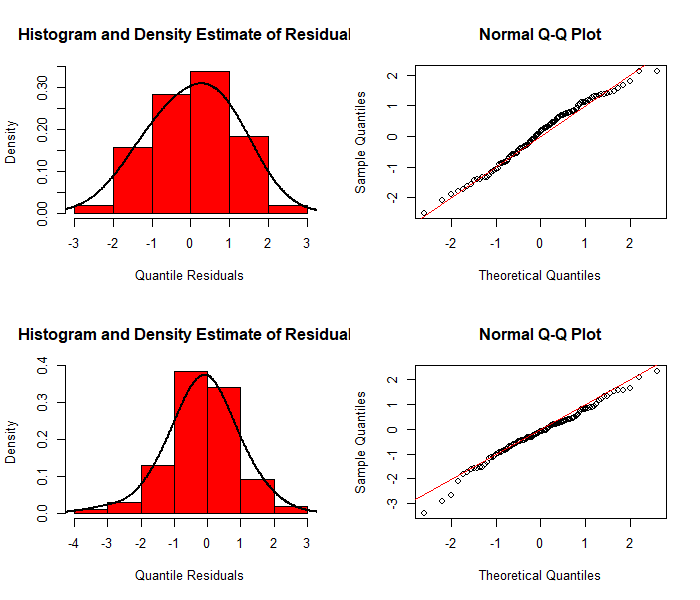
\includegraphics[width=0.95\linewidth]{figures/res_hist_qqplot_26.png}
  \caption{Diagnostic plots of quantile residuals based on \ac{GJRM} models for key category clusters 2 \& 6}
  \label{fig:res_hist_qqplot_26}
\end{figure}



The effect of time on the copula parameter turns out to be significant (R output \ref{output:summary_kcc_26} and can be viewed in \autoref{fig:time_effect_on_theta_26}, where the number 26.64 in brackets on the y-axis denotes the effective degrees of freedom of the smooth curve, which is centered around zero due to identifiability constraints.
\\

\begin{figure}[H]
\centering
  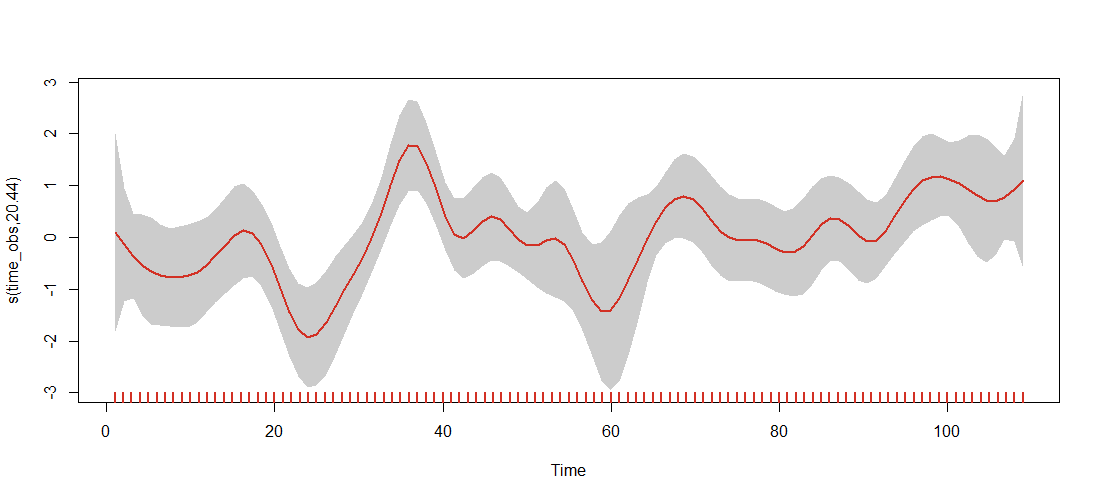
\includegraphics[width=0.95\linewidth]{figures/time_effect_on_theta_26.png}
  \caption{Estimated Smooth effect of time on the copula parameter $\theta$ with 95\% confidence bands for key category clusters 2 \& 6}
  \label{fig:time_effect_on_theta_26}
\end{figure}



\begin{figure}[H]
\centering
  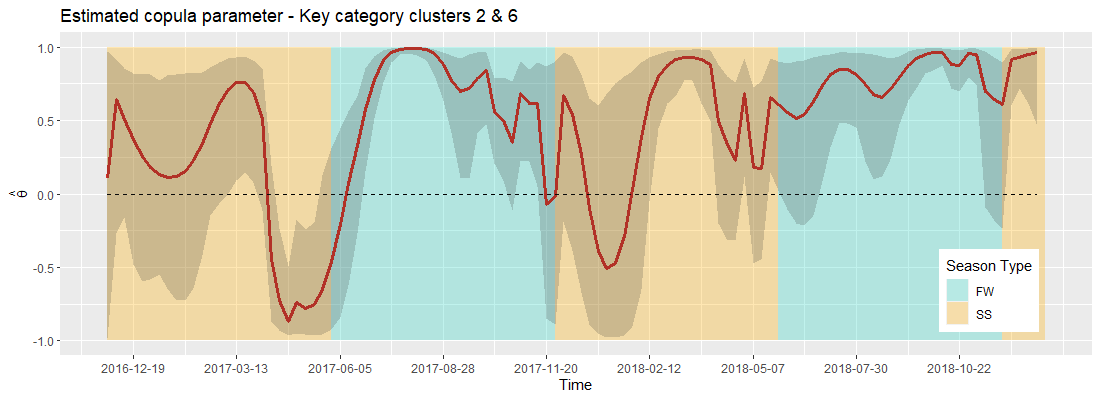
\includegraphics[width=0.95\linewidth]{figures/estimated_theta_kcc_26.png}
  \caption{Estimated copula parameter over time and 95\% confidence bands from a \ac{GJRM} t-copula model with normal margins for key category clusters 2 \& 6 - Season type in the background - Dashed horizontal line at $\hat{\theta} = 0$}
  \label{fig:estimated_theta_kcc_26}
\end{figure}
%  - Confidence bands are neglected for clarity of the graph

\autoref{fig:estimated_theta_kcc_26} displays the correlation between the two margins which highly fluctuates between (almost) perfect negative and positive dependence, suggesting that only copulas which can account for both of those dependence (concordance) types should be considered. Candidate copulas were the Frank copula, the Ali-Mikhali-Haq copula and Fari-Gumbel-Morgenstern copula, where the last two can only account for weak dependencies \citep{marra1605bivariate}. The Student's t-copulas provides the most appropriate fit among those types of copulas so we stick to it. The width of the confidence intervals also does vary a lot across different parts of the observation period. \\

Positive correlation in a business context would mean that for both clusters sales are increasing conjointly. Negative correlations (below dashed line of \autoref{fig:estimated_theta_kcc_26}) indicate that as one's cluster's sales increase the other one's drop and further questioning should be carried out. We see such negative correlations during the Spring-Summer seasons and somewhat during Black Friday towards the end of Fall-Winter 2017.


%We will start the pairwise analysis with inspecting the \ac{GJRM} approach. As mentioned above, the margins are specified as Dagum distributed \acp{RV} and we choose the Student's t copula (the degrees of freedom do not affect the outcome, as they just serve as starting values for \ac{GAMLSS} estimation). All model parameters are set to constant, except the copula parameter (which is defined as in \autoref{eq:gjrm_kcc}). These settings also hold for Subsections \ref{sssec:kcc_28} and \ref{sssec:kcc_68}. We can see in the diagnostic plots of \autoref{fig:margin_estimates_kcc_26} that this type of model fitting returns quite successful results. \\
%
%\begin{figure}[H]
%\centering
%  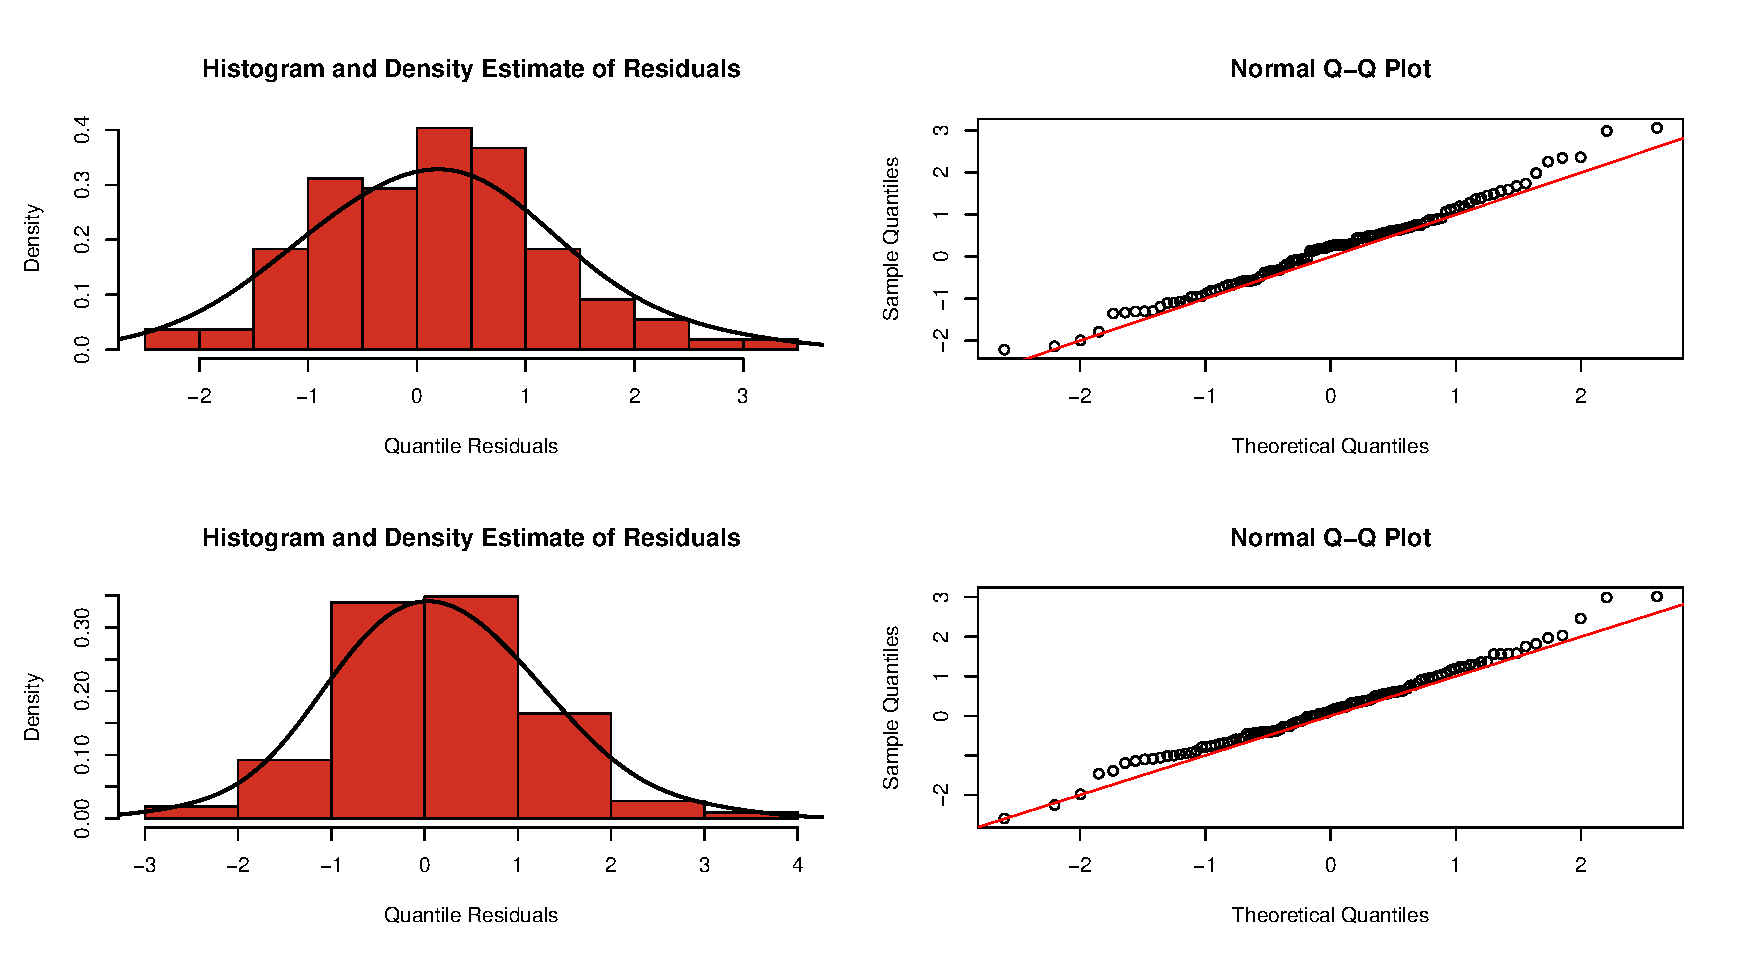
\includegraphics[width=0.9\linewidth]{figures/margin_estimates_kcc_26.eps}
%  \caption{Estimation diagnostics for the response margins KCC 2 \& KCC 6; \ac{GJRM} approach}
%  \label{fig:margin_estimates_kcc_26}
%\end{figure}
%
%Regarding the fitting of the copula parameter $\rho$, time-varying estimation is achieved. The red line in \autoref{fig:copula_parameters_26} shows the estimated time-dependent sequence of $\hat{\rho}$, where an instant positive conclusion is that the outcome is very close to the gamCopula approach. This indicates that the model setup of these two approaches both agree for the most part on the dependence structure. (Confidence intervals of the lines are not shown to retain clarity in the figure).\\
%
%
%\begin{figure}[H]
%\centering
%  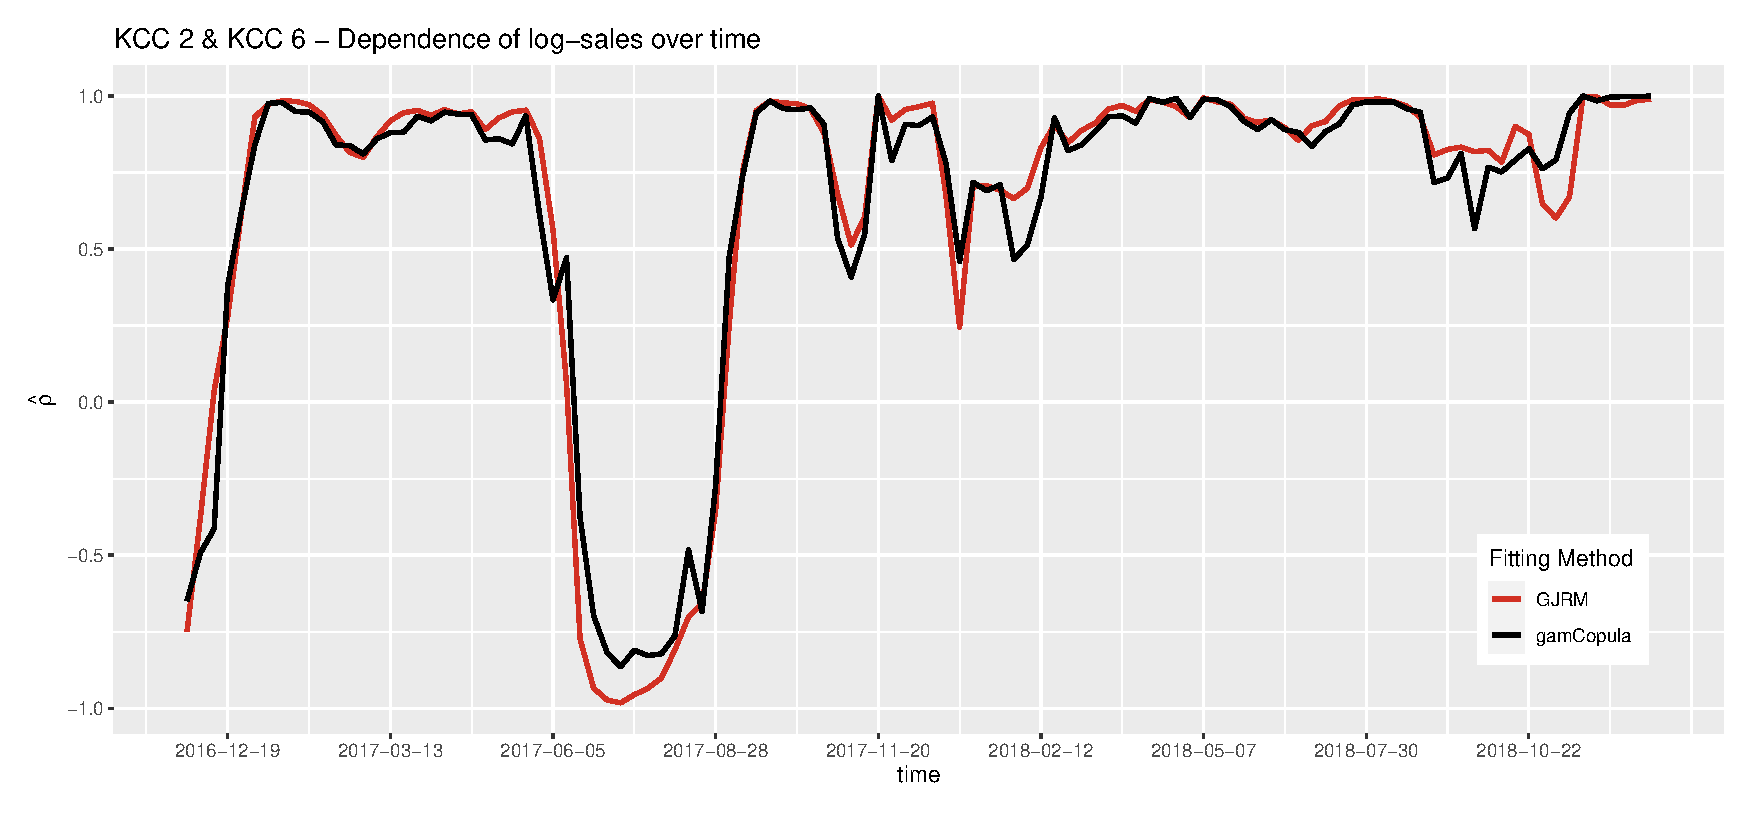
\includegraphics[width=0.9\linewidth]{figures/copula_parameters_26.eps}
%  \caption{Estimated time-varying Pearson's correlation coefficients for the pair KCC 2 \& KCC 6}
%  \label{fig:copula_parameters_26}
%\end{figure}
%
%
%By large, the dependence is constantly at a very high positive level, with a noticeable turn in high negativity during the summer months of 2017. The gamCopula approach seems to pick up slightly more regional fluctuations than the \ac{GJRM} approach.






